%
%  長野高専 電子情報工学科 卒業研究発表会 予稿スタイルファイル
%  Version 2019
%
%  作成: 伊藤祥一
%  協力: 大矢健一
%
\documentclass[a4j, 9pt, twocolumn, twoside]{jsarticle}
\usepackage{eipaper}

%  タイトル・著者・指導教員
\newcommand{\Jtitle}{機械学習を用いた天気予報システムの作成}
\newcommand{\JtitleShort}{\Jtitle} % 短縮する場合は\newcommand{\JtitleShort}{わが猫}のようにする
\newcommand{\Etitle}{Creating a weather forecast system using machine learning}
\newcommand{\Author}{清水 翔仁}  %  姓と名の間に半角スペース
\newcommand{\Teacher}{大矢 健一}

%  年度と発表月の設定
\newcommand{\Nendo}{2019}  %  年度
\newcommand{\Happyo}{1}    %  2019年度の1月(=2020年1月)に発表会
\setcounter{Nanki}{\number\Nendo}
\addtocounter{Nanki}{-1992}
\setcounter{HappyoYear}{\number\Nendo}
\addtocounter{HappyoYear}{1}

%  ページ番号の設定
\newcommand{\LabSymbol}{B}  % B-5からはじめる
\setcounter{page}{5}


%
%  本文
%
\begin{document}
\twocolumn[\Maketitle]\footnotetext[1]{指導教員: \Teacher}
\section{そもそも予稿集に何を書くべきか}
予稿集の執筆にあたっては,読者として想定される2通りの人々,すなわち発
表会会場に来ている人とそうでない人の両方に対する配慮が必要である.前者
に対しては,学会などでは通常いくつもの部屋を使って同時進行でいくつもの
発表が行われるということを踏まえた配慮をしなければならない.この読者に
とって予稿集は「その発表を聞きに行くべきか」という判断材料として使われ
る.後者に対する配慮としては,来られない人が予稿集を読むことで,その研
究の概要と得られた知見を一通り知ることができるようにしておくことが必要
である.いずれの場合においても,問題意識・アプローチ方法・得られた結果
や知見(考察)が簡潔にまとまっていることが必要である.また,明文化はされ
ていないが,慣習として与えられたページのほぼ末尾まで埋めることがマナー
である.

\section{スタイルファイルの使い方}
ここでは電子情報工学科予稿集スタイルファイルの使い方について述べる.

\subsection{一般的な注意事項}
会議の議事録などとは違い,予稿集をはじめとする論文集の体裁には伝統的か
つ「堅い」約束事が数多くある.そのためスタイルファイルも「堅い」ものと
なっており,\LaTeX の特徴の一つであるカスタマイズ機能は大幅に制限さ
れる.例えば\texttt{\textbackslash textheight}などのいわゆる
スタイルパラメータを変更する
のは当然やめていただきたい.どのようなカスタマイズが許されるのかを示す
のは難しいが,一つの基準として「スタイルファイルを読んでみて大丈夫だと
確信が持てる」こと以外はしないことを強く勧める.
なお,これらの変更やこのガイドで述べている「やめて欲しいこと」を行なっても,
\textbf{エラーになったりせず単に結果が変になる}ことに注意していただきたい.

\subsection{論文の構成}\label{sec:config}
ファイルは次の形式で作る.
\begin{quote}\small
\texttt{\textbackslash documentstyle[a4j, 10pt, twocolumn, twoside]\{jsarticle\}}\\
\texttt{\textbackslash usepackage\{new\}}\\
年度と発表月,ページ番号を設定する.\\
\texttt{\textbackslash newcommand\{\textbackslash Nendo\}\{2016\}}\\
\texttt{\textbackslash newcommand\{\textbackslash Happyo\}\{2\}}\\
\texttt{\textbackslash newcommand\{\textbackslash LabSymbol\}\{B\}}\\
\texttt{\textbackslash setcounter\{page\}\{5\}}\\
必要ならばユーザのマクロ定義などをここに書く.\\
\texttt{\textbackslash JTitle\{日本語表題\}}\\
\texttt{\textbackslash JTitleShort\{日本語表題(短縮)\}}\\
\texttt{\textbackslash Etitle\{英語表題\}}\\
\texttt{\textbackslash Author\{学生氏名\}}\\
\texttt{\textbackslash Teacher\{教員氏名\}}\\
\texttt{\textbackslash begin\{document\}}\\
\texttt{\textbackslash twocolumn[\textbackslash Maketitle]}\\
\texttt{\textbackslash section\{$\langle$第1節の表題$\rangle$\}}\\
\quad $\ldots\ldots\ldots$\\
\quad$\langle$本文$\rangle$\\
\quad $\ldots\ldots\ldots$\\
\texttt{\textbackslash begin\{thebibliography\}\{9\}}\\
\quad $\ldots\ldots\ldots$\\
\texttt{\textbackslash end\{thebibliography\}}\\
\texttt{\textbackslash end\{document\}}
\end{quote}

\subsection{オプション・スタイル}
オプションのスタイルファイルによっては予稿集スタイルと矛盾するようなも
のもあるので,スタイルファイルの性格を良く理解して使用していただきたい.

\subsection{巻数,号数などの記述}
今年度の西暦年を\texttt{\textbackslash Nendo}に,
卒研発表会の行われる月を\texttt{\textbackslash Happyo}に,
それぞれ設定する.ページ左上のVol.等は自動計算される.
\begin{quote}\small
\verb+\newcommand{\Nendo}{2019}+
\verb+\newcommand{\Happyo}{1}+
\end{quote}

また,ページのブロック番号が卒研室ごとにA, B, ...と
事前打ち合わせで割り振られているのでこれを
\verb+\LabSymbol+に設定する.卒研室内での発表順に
従って1から割り振ったページ番号を
\verb+\setcounter{page}{5}+の5という部分に設定する.

\begin{quote}\small
\verb+\newcommand{\LabSymbol}{B}+
\verb+\setcounter{page}{5}+
\end{quote}

\subsection{表題などの記述}\label{sec:Desc}\label{sec:DESC}
表題,英文表題,著者名とその所属を前述のコマンドや環境により定義した後,
\texttt{\textbackslash Maketitle}によって出力する.

\begin{description}
\item[表題]{\verb+\Jtitle+および\verb+\Etitle+で定義した表題はセンタリングされる.
なお和文表題は奇数ページのヘッダにも表示されるので,ヘッダに納まらないような
長い表題の場合のみ
\begin{quote}\small
\verb+\JtitleShort{ヘッダ用表題}+
\end{quote}
のようにヘッダ用に短くしたものを指定する.}
\item[著者名と指導教員]{著者名と指導教員をそれぞれ
\begin{quote}\small
\verb+\Author{著者名}+\\
\verb+\Teacher{指導教員名}+
\end{quote}
なお,著者名・指導教員名とも必ず\textbf{姓と名を半角の空白で区切る}.}
\end{description}

\subsection{見出し}
節や小節の見出しには \verb+\section+, \verb+\subsection+といった
コマンドを使用する.簡潔でわかりやすい見出しとなるよう心がける.

\subsection{文章の記述}
\begin{description}
\item[行送り]{予稿集は2段組を採用しており,左右の段で行の基準線の位置が
一致することを原則としている.また,節見出しなど,行の間隔を他より
たくさんとった方が読みやすい場所では,この原則を守るようにスタイルファイルが自動的にス
ペースを挿入する.したがって本文中では \verb+\vspace+や\verb+\vskip+を
用いたスペースの調整を行なわないでいただきたい.}
\item[フォントサイズ]{このガイドの印刷結果からもわかるように,予稿集
スタイルでは様々な大きさのフォントが使われるが,これらはすべて
スタイルファイルが自動的かつ注意深く選択したものである.したがって,
著者が自分でフォントサイズを変更する必要はなく,かえって行送りの
原則を守る妨げにもなるため可能な限り手動での変更は避ける.}
\item[句読点]{句点には全角の「.」,読点には全角の「,」をなるべく用いる.ただし英文
中や数式中で「.」や「,」を使う場合には,半角文字を使い,直後に半角
スペースを1つ入れる.「.」や「,」は,なるべくならば一切使わない.}
\item[全角文字と半角文字]{
全角文字と半角文字の両方にある文字は次のように使い分ける.
\begin{enumerate}
\item{括弧は全角の「(」と「)」を用いる.但し,書誌データでは
半角の「(」と「)」を用いる.}
\item{英数字,空白,記号類は半角文字を用いる.
ただし,句読点に関しては,前項で述べたような例外がある.}
\item{カタカナは全角文字を用いる.}
\item{引用符では開きと閉じを区別する. 開きには \verb+``+(``)
を用い,閉じには \verb+''+('')を用いる.}
\end{enumerate}
}
\end{description}

\subsection{数式}
\begin{description}
\item[本文中の数式]{
本文中の数式は\texttt{\$}と\texttt{\$}で囲む.
なお$\frac{a}{b}$~(\texttt{\textbackslash frac\{a\}\{b\}}) のように
背が高い要素は見苦しくかつ行送りを乱すことにもなるので,
使用しないようにしていただきたい.}
\item[別組の数式]{別組数式(displayed math)については
\textbf{\$\$〜\$\$は使用してはならない}.
すなわち\verb+\[+と\verb+\]+で囲むか,
\texttt{\textbackslash displaymath}, \texttt{\textbackslash equation}, 
\texttt{\textbackslash eqnarray}のいずれかの環境を
用いなければならない.これらは
\begin{equation}
\Delta_l = \sum_{i=l+1}^L\delta_{pi}
\end{equation}
のように,センタリングではなく固定字下げで数式を出力し,
かつ背が高い数式による行送りの乱れを吸収する機能がある.}
\item[eqnarray環境]{
互いに関連する別組の数式が2行以上連続して現れる場合には,
単に\verb+\[+と\verb+\]+,
あるいは \texttt{\textbackslash begin\{equation\}}と
\texttt{\textbackslash end\{equation\}}で囲った数式を書き並べるのではなく,
\texttt{\textbackslash begin\{eqnarray\}}と
\texttt{\textbackslash end\{eqnarray\}}を使って,
等号(あるいは不等号)の位置で縦揃えを行なった方が読みやすい.}
\item[数式のフォント]{\LaTeX が標準的にサポートしているもの以外の
特殊な数式用フォントは,できるだけ使わないようにしていただきたい.}
\end{description}

\subsection{図}
図は次の形式で指定する. 位置の指定に\texttt{h}
は使わない.文字数が多い見出しは自動的に改行して最大幅の行を
基準にセンタリングするが,見出しが2行になる場合には適宜
~\verb+\\+~を挿入して改行したほうが良い結果となることがしばしばある.
図の参照には\texttt{\textbackslash figref\{ラベル\}}を用いると,
\figref{fig-search}のようになる.

\begin{figure}
\centering
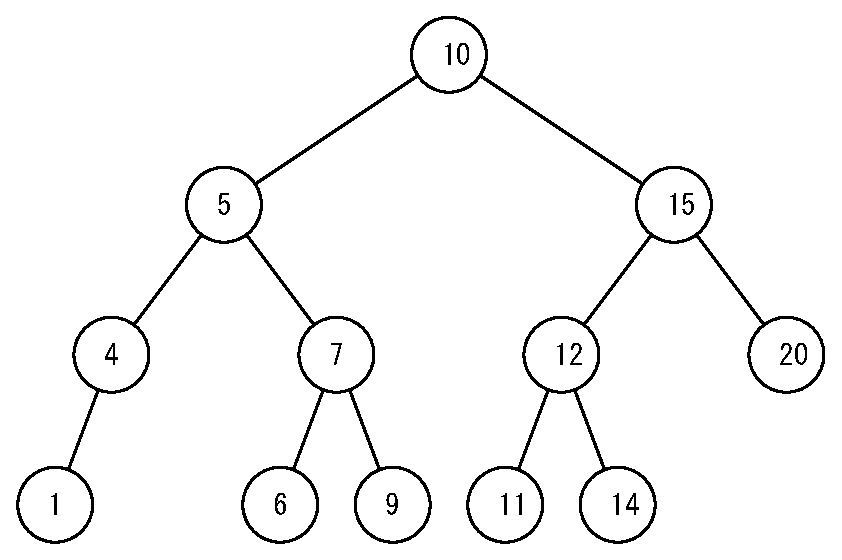
\includegraphics[scale=0.5]{search.eps}
\caption{2分探索木}
\label{fig-search}
\end{figure}

\begin{quote}\small
\verb+\begin{figure}+\\
\verb+\centering+\\
\verb+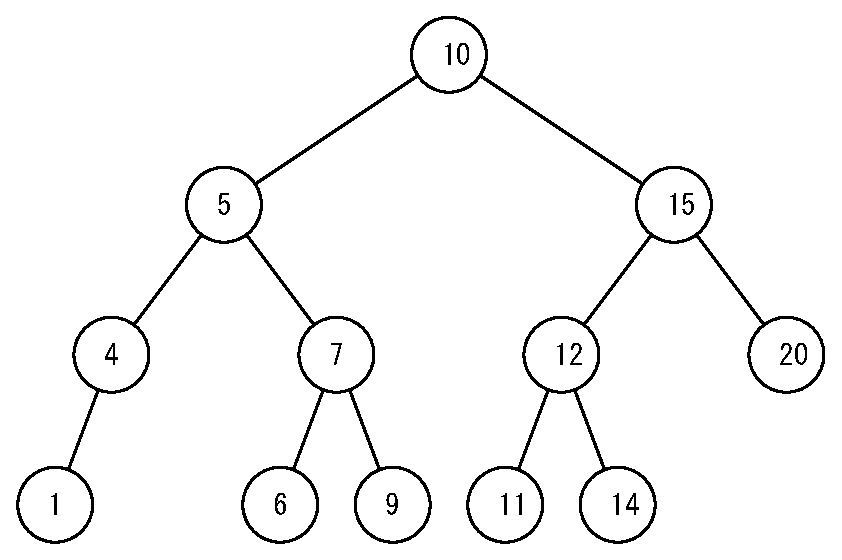
\includegraphics[scale=0.5]{search.eps}+\\
\verb+\caption{2分探索木}+\\
\verb+\label{fig-search}+\\
\verb+\end{figure}+
\end{quote}

図の中では本文と違い,どのような大きさのフォントを使用しても構わない.
EPSファイル自体はカラーも扱うことができるが,印刷時には白黒になってし
まうことに注意.また,小さな記号や細い線は印刷時に判読不能になってしま
うこともある.

\subsection{表}
表の罫線はなるべく少なくするのが,仕上がりをすっきりさせるコツである.罫線を
つける場合には,一番上の罫線には二重線を使い,左右の端には縦の罫線をつけない 
(\tabref{tbl-jinko}).
また,表の\textbf{上}に見出しを\texttt{\textbackslash caption}
で指定する.表の参照は\texttt{\textbackslash tabref\{ラベル\}}を用いて行なう.

\begin{table}\small
\centering
\caption{長野県の市町村別人口~\cite{jinko}}
\label{tbl-jinko}
\begin{tabular}{c|r|r|r}
\hline\hline
市町村名 & 人口総数(人) & 男性(人) & 女性(人) \\ \hline
長野市 & 376,072 & 181,553 & 194,519 \\
松本市 & 241,287 & 118,314 & 122,973 \\
上田市 & 155,891 & 75,963 & 79,928
\end{tabular}
\end{table}


\subsection{箇条書}\label{sec:item*}
予稿集では箇条書に関する形式を特に定めておらず,
場合に応じて様々な様式が用いられている.

\subsection{脚注}
脚注は\texttt{\textbackslash footnote}コマンドを使って書くと,
ページ単位に\footnote{脚注の例.}や\footnote{二つめの脚注.}のような
参照記号とともに脚注が生成される.

\subsection{参考文献の参照}
本文中で参考文献を参照する場合には,参考文献番号が文中の単語として使わ
れる場合と,そうでない参照とでは,使用する文字の大きさが異なる.前者は
\verb+\Cite+により参照し,後者は\verb+\cite+により参照する.たとえば;

\begin{quote}
文献\verb+\Cite{latex}+は\verb+\LaTeX\cite{latex}+の総合的な解説書である.
\end{quote}
と書くと
\begin{quote}
文献\Cite{latex}は\LaTeX\cite{latex}の総合的な解説書である.
\end{quote}
が得られる.

また,一つの \verb+\Cite+あるいは\verb+\cite+コマンドで
三つ以上の文献を参照し,かつそれらの参照番号が連続している場合,
\Cite{latex, bibunsho, jinko}や
「文献\cite{latex, bibunsho, jinko}」のように,
自動的に先頭と末尾の文献番号が\ $--$\ で結合される.

\subsection{参考文献リスト}
参考文献リストには,原則として本文中で引用した文献のみを列挙する.
順序は参照順あるいは第一著者の苗字のアルファベット順とする.
Webページは数年後に閲覧できる保証はないので,参考文献には
URLを可能な限り含めない.
このガイドの参考文献リストを注意深く見て,
そのスタイルにしたがっていただきたい.

\section{拡張機能の使い方}
okumacro.styが読み込まれているので,
\begin{quote}\small
\verb+\ruby{沈丁花}{じんちょうげ}+\\
\verb+\kenten{圏点}+
\end{quote}
とすると\ruby{沈丁花}{じんちょうげ}のようにルビや\kenten{圏点}を
振ることができる.
okumacro.styの概説については文献~\Cite{bibunsho}を参照のこと.

\begin{thebibliography}{9}
\bibitem{latex}{Leslie Lamport(著), 大野俊治・藤浦はる美・倉沢良一・小暮博道・Edgar Cooke(訳): 文書処理システム\LaTeX, アスキー, 1990.}
\bibitem{jinko}{毎月人口異動調査(平成28年3月1日現在): \url{http://www3.pref.nagano.lg.jp/tokei/1_jinkou/jinkou.htm}}
\bibitem{bibunsho}{奥村晴彦・黒木裕介: [改訂第7版] LaTeX2e 美文書作成入門, 技術評論社, 2017.}
\end{thebibliography}
\end{document}
